\documentclass[border=3pt]{standalone}
% Preâmbulo compartilhado pelos diagramas TikZ da aula 4 de Navegação (Representação de Mapas)
\usepackage[T1]{fontenc}
\usepackage[utf8]{inputenc}
\usepackage{lmodern}
\usepackage{amsmath}
\usepackage{xcolor}
\usepackage{tikz}
\usetikzlibrary{arrows.meta,angles,quotes,decorations.pathmorphing,decorations.pathreplacing,calc,
                positioning,shapes.geometric,shapes.misc,backgrounds,fit,
                math}

% Paleta (mesma dos SVGs originais)
\definecolor{dblue}{HTML}{2A5B8C}
\definecolor{dorange}{HTML}{B3541E}
\definecolor{dgreen}{HTML}{4A7C59}
\definecolor{dred}{HTML}{9C4B4B}
\definecolor{dcream}{HTML}{F4F1EA}
\definecolor{dshade}{HTML}{DDD7C9}

% Função gaussiana (não normalizada por padrão de escala visual)
\pgfmathdeclarefunction{gauss}{3}{%
  \pgfmathparse{1/(#3*sqrt(2*pi))*exp(-((#1-#2)^2)/(2*#3^2))}%
}

% Estilos comuns (prefixo d... para não colidir com chaves internas do pgf)
\tikzset{
  >={Stealth[length=2mm]},
  dguide/.style={gray!55, dashed, line width=0.4pt},
  daxis/.style={gray!60, line width=0.7pt, ->},
  dbody/.style={fill=black!3, draw=black!80, line width=1pt},
  dacc/.style={draw=dblue, line width=1pt},
  dlbl/.style={black!55, font=\small},
  dsub/.style={black!45, font=\footnotesize},
  dstate/.style={circle, draw=black!80, fill=dcream, line width=1pt,
                 minimum size=17mm, font=\large, inner sep=1pt},
  dobs/.style={circle, draw=black!80, fill=dshade, line width=1pt,
               minimum size=14mm, font=\large, inner sep=1pt},
  dbox/.style={rounded corners=2pt, draw=black!80, fill=dcream, line width=1pt,
               align=center, inner sep=6pt},
  dop/.style={circle, draw=black!80, fill=white, line width=1pt,
              minimum size=6mm, inner sep=0pt, font=\small},
  dtrans/.style={->, dblue, line width=1pt},
  dmeas/.style={->, dorange, line width=1pt},
  dcurve/.style={line width=1pt, dblue},
  dcurveb/.style={line width=1.4pt, dorange},
}

\begin{document}
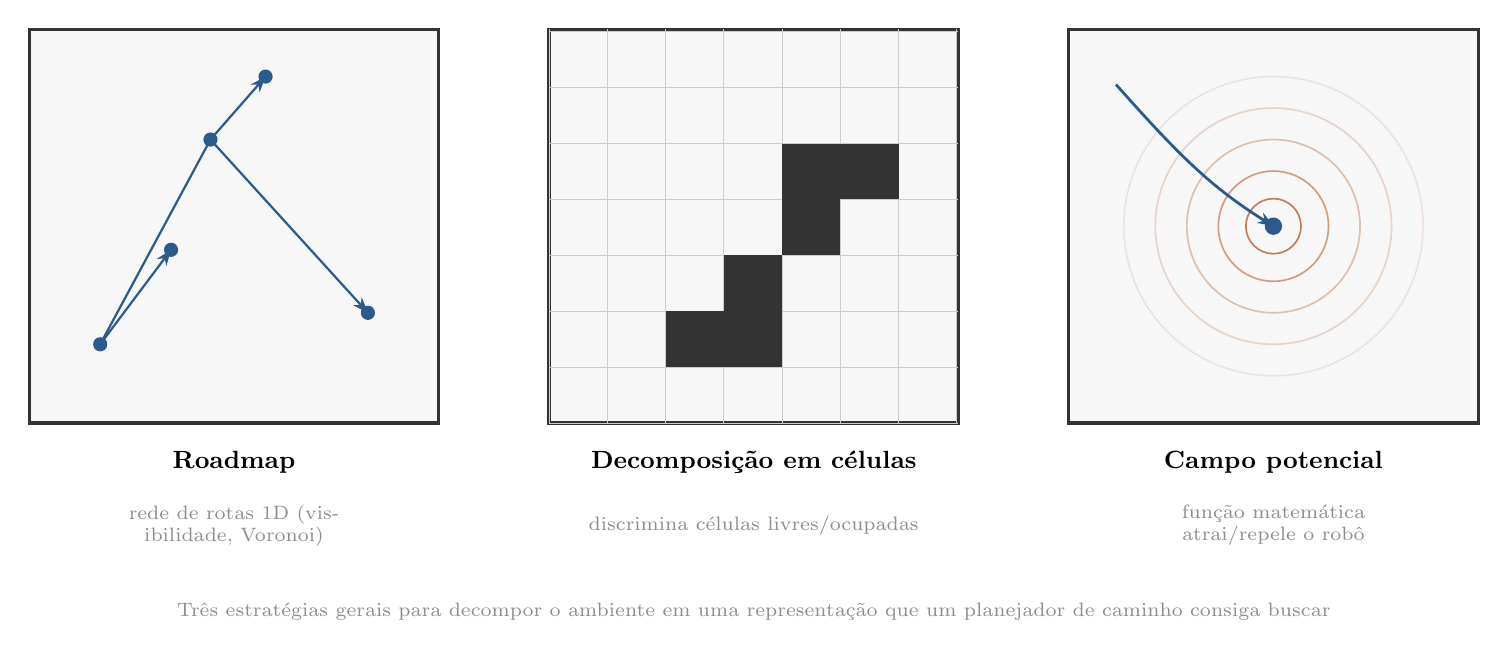
\begin{tikzpicture}[x=1cm,y=1cm]

  % Card 1: Roadmap
  \begin{scope}[shift={(0,0)}]
    \draw[dbody, line width=1.2pt] (0,0) rectangle (5.2,5.0);
    \draw[dtrans, line width=0.8pt] (0.9,1.0) -- (2.3,3.6) -- (4.3,1.4);
    \draw[dtrans, line width=0.8pt] (2.3,3.6) -- (3.0,4.4);
    \draw[dtrans, line width=0.8pt] (0.9,1.0) -- (1.8,2.2);
    \foreach \p in {(0.9,1.0),(2.3,3.6),(4.3,1.4),(3.0,4.4),(1.8,2.2)}
      \fill[dblue] \p circle (0.09);
    \node[font=\bfseries\small] at (2.6,-0.5) {Roadmap};
    \node[dsub, font=\scriptsize, align=center, text width=4.6cm] at (2.6,-1.3) {rede de rotas 1D (visibilidade, Voronoi)};
  \end{scope}

  % Card 2: Decomposição em células
  \begin{scope}[shift={(6.6,0)}]
    \draw[dbody, line width=1.2pt] (0,0) rectangle (5.2,5.0);
    \foreach \x in {0,0.74,...,5.2} { \draw[black!20, line width=0.3pt] (\x,0) -- (\x,5.0); }
    \foreach \y in {0,0.71,...,5.0} { \draw[black!20, line width=0.3pt] (0,\y) -- (5.2,\y); }
    \foreach \x/\y in {1.48/0.71,2.22/0.71,2.22/1.42,2.96/2.13,2.96/2.84,3.7/2.84} {
      \fill[black!80] (\x,\y) rectangle ++(0.74,0.71);
    }
    \node[font=\bfseries\small] at (2.6,-0.5) {Decomposição em células};
    \node[dsub, font=\scriptsize, align=center, text width=4.6cm] at (2.6,-1.3) {discrimina células livres/ocupadas};
  \end{scope}

  % Card 3: Campo potencial
  \begin{scope}[shift={(13.2,0)}]
    \draw[dbody, line width=1.2pt] (0,0) rectangle (5.2,5.0);
    \foreach \r/\o in {1.9/12,1.5/22,1.1/35,0.7/55,0.35/75} {
      \draw[dorange, line width=0.6pt, opacity=\o/100] (2.6,2.5) circle (\r);
    }
    \fill[dblue] (2.6,2.5) circle (0.11);
    \draw[dtrans, -{Stealth[length=2mm]}] (0.6,4.3) .. controls (1.4,3.4) and (1.8,3.0) .. (2.6,2.5);
    \node[font=\bfseries\small] at (2.6,-0.5) {Campo potencial};
    \node[dsub, font=\scriptsize, align=center, text width=4.6cm] at (2.6,-1.3) {função matemática atrai/repele o robô};
  \end{scope}

  \node[dsub, font=\scriptsize, align=center, text width=17.5cm] at (9.2,-2.4)
     {Três estratégias gerais para decompor o ambiente em uma representação que um planejador de caminho consiga buscar};

\end{tikzpicture}
\end{document}
